\documentclass{article}

\usepackage{arxiv}

\usepackage[utf8]{inputenc} % allow utf-8 input
\usepackage[T1]{fontenc}    % use 8-bit T1 fonts
\usepackage{lmodern}        % https://github.com/rstudio/rticles/issues/343
\usepackage{hyperref}       % hyperlinks
\usepackage{url}            % simple URL typesetting
\usepackage{booktabs}       % professional-quality tables
\usepackage{amsfonts}       % blackboard math symbols
\usepackage{nicefrac}       % compact symbols for 1/2, etc.
\usepackage{microtype}      % microtypography
\usepackage{graphicx}
\usepackage{amsmath}
\usepackage{float}
\usepackage{enumitem}
\usepackage{subcaption}
\usepackage[backend=biber,style=authoryear]{biblatex}
\addbibresource{reference.bib}

\title{Replication of Crypto Factor Analysis}

\author{
    \small
    \begin{minipage}[t]{0.24\textwidth}
        \centering
        Daniel Liang \\
        Master of Science in Finance \\
        University of Illinois \\
        \texttt{\href{mailto:yuanhui5@illinois.edu}{\nolinkurl{yuanhui5@illinois.edu}}}
    \end{minipage}
    \hfill
    \begin{minipage}[t]{0.24\textwidth}
        \centering
        Zixuan Feng \\
        Master of Science in Finance \\
        University of Illinois \\
        \texttt{\href{mailto:zf20@illinois.edu}{\nolinkurl{zf20@illinois.edu}}}
    \end{minipage}
    \hfill
    \begin{minipage}[t]{0.24\textwidth}
        \centering
        Xiyu Cai \\
        Master of Science in Finance \\
        University of Illinois \\
        \texttt{\href{mailto:xiyucai2@illinois.edu}{\nolinkurl{xiyucai2@illinois.edu}}}
    \end{minipage}
    \hfill
    \begin{minipage}[t]{0.24\textwidth}
        \centering
        Weihua Zhang \\
        Master of Science in Finance \\
        University of Illinois \\
        \texttt{\href{mailto:weihuaz2@illinois.edu}{\nolinkurl{weihuaz2@illinois.edu}}}
    \end{minipage}
}


% tightlist command for lists without linebreak
\providecommand{\tightlist}{%
  \setlength{\itemsep}{0pt}\setlength{\parskip}{0pt}}


% Pandoc citation processing
\newlength{\cslhangindent}
\setlength{\cslhangindent}{1.5em}
\newlength{\csllabelwidth}
\setlength{\csllabelwidth}{3em}
\newlength{\cslentryspacingunit} % times entry-spacing
\setlength{\cslentryspacingunit}{\parskip}
% for Pandoc 2.8 to 2.10.1
\newenvironment{cslreferences}%
  {}%
  {\par}
% For Pandoc 2.11+
\newenvironment{CSLReferences}[2] % #1 hanging-ident, #2 entry spacing
 {% don't indent paragraphs
  \setlength{\parindent}{0pt}
  % turn on hanging indent if param 1 is 1
  \ifodd #1
  \let\oldpar\par
  \def\par{\hangindent=\cslhangindent\oldpar}
  \fi
  % set entry spacing
  \setlength{\parskip}{#2\cslentryspacingunit}
 }%
 {}
\usepackage{calc}
\newcommand{\CSLBlock}[1]{#1\hfill\break}
\newcommand{\CSLLeftMargin}[1]{\parbox[t]{\csllabelwidth}{#1}}
\newcommand{\CSLRightInline}[1]{\parbox[t]{\linewidth - \csllabelwidth}{#1}\break}
\newcommand{\CSLIndent}[1]{\hspace{\cslhangindent}#1}

\begin{document}
\maketitle


\begin{abstract}
% This study utilizes almost stochastic dominance (AFSD and ASSD) to assess portfolio strategies based on momentum and size factors against the S\&P 500 benchmark over 1 to 78 weeks. Short-term analysis reveals that momentum strategies (rmom1, rmom3, rmom4, rmom8) perform better with short-only portfolios, which consistently dominate long-only portfolios under AFSD and ASSD. For longer-term horizons (52 and 78 weeks), size-based strategies show significant outperformance, with long-only portfolios surpassing the benchmark. Our analysis supports the value of incorporating short positions in portfolio management, particularly for momentum strategies, and suggests that size factors can be effective for long-term investment horizons.
\end{abstract}

\keywords{
    trading strategies
   \and
    quantitative analysis
   \and
    cryptocurrency
   \and
    stochastic dominance
  }

\hypertarget{introduction}{%
\section{Introduction}\label{introduction}}

Cryptocurrencies such as Bitcoin are virtual assets that are usually not cleared on centralized exchanges, ensuring their transparency and preventing them from being easily stolen and attacked. In the past few years, these assets have caught the increasing attention of investors because of their extraordinary returns, volatility, and leverage. Two of the most widely discussed topics for them are pricing models and investing preferences over other asset classes. 

Because of their vague intrinsic values and virtual designs, some fundamental analyses that apply to common equities will not work for them. Wang and Chong (2021) extended the traditional Fama–French three-factor model to replace the value-to-growth factor with the coin-to-token factor as a proxy and include some volatility, liquidity and macro factors. Poongodi et al. (2020) tried to use market data and some machine learning models, such as linear regression and support vector machine, to make some price predictions of Ethereum. Although these two pieces of research investigate the fair price of cryptocurrencies from two distinct angles, fundamental factors and market technical analysis, there is still a huge room for rational investors to dig into the fair value discovery of these virtual assets.

Besides, many investors are trying to figure out whether cryptocurrency will be a good choice for mid to long-term investments over other investment options, such as bonds and stocks. Because of the non-normal distribution of returns, Han et al. (2021) adopted one non-parametric method, almost stochastic dominance, to compare the performances of factor portfolios of cryptocurrencies to those of stock indexes and bonds.

This report replicates the findings of Han et al. (2021) on cryptocurrency factor portfolios, using data from Wharton Research Data Services (WRDS) and Binance. Following the original methodology, we analyze market data for 82 cryptocurrencies (2014-2024) and trading data for 10 cryptocurrencies (2017-2024). The study employs R to validate the original conclusions on portfolio performance and dominance over traditional financial benchmarks, examining the roles of risk premiums and mispricing.

This paper is organized as follows. {\bf Section 2} summarises the paper intended to replicate, {\em Cryptocurrency Factor Portfolios: Performance, Decomposition and Pricing Models} by Han et al. (2021), and discusses some of their interesting findings. {\bf Section 3} reviews relevant literature and research on our topics, such as factor models and almost stochastic dominance. {\bf Section 4} describes the data and summary statistics. {\bf Section 5} presents the results generated by similar approaches adopted by Han et al. (2021) with the data described in {\bf Section 4}. {\bf Section 6} discusses some limitations and potential downsides of this project and provides some guidelines for future improvements. {\bf Section 7} concludes this project and compares our findings to those of Han et al. (2021). 

\hypertarget{paper-summary}{%
\section{Paper Summary}\label{paper-summary}}

Han et al. (2021) argued that cryptocurrency factor portfolios outperform traditional assets, through a combination of almost stochastic dominance (ASD) and factor modelling. The ASD method includes almost first-degree stochastic dominance (AFSD) and almost second-degree stochastic dominance (ASSD), addressing the limitations of traditional metrics, such as mean-variance analysis, to non-normal distributions of returns, which was proven by the paper. AFSD will examine whether a portfolio is preferred without knowledge of investors' risk tolerances, while ASSD will assume the investors are risk-averse to analyse the dominance of a portfolio over another. To identify dominance, the paper set critical thresholds at 5.9\% for AFSD and 3.2\% for ASSD.

The study constructed 27 factors, divided into 4 main categories - size, momentum, volume and volatility - shown in {\bf Table 1} in {\bf Section 5}. They divided each factor into 5 quantiles respectively, examined the returns of each quantile, and constructed a long-short portfolio by longing the quantile and shorting quantile 1 with weights based on market capitalization. Then, they utilized ASD to compare these factor portfolios' performances to those of S\&P 500, of 10-year U.S, of 1-month T-bill and of the cryptocurrency index. Treasury bonds, with five different holding periods, 4-week, 13-week, 26-week, 52-week and 78-week. For the S\&P 500, no dominance was found for the holding periods of 4-week and 13-week. Ten factors (LPRC, MAXPRC, MOM1, MOM2, MOM3, ROMO1, RMOM2, RMOM3, RMOM4 and STDPRCVOL) showed AFSD and five of them (LPRC, MAXPRC, MOM1, MOM3 and RMOM2) showed ASSD for longer holding horizon. Extending the investment horizon, an increasing number of factors showed dominance, as high returns would compensate for the high volatility. For 52-week, besides of above factors, seven new factors (MARCAP, VOLPRC, VOLSCALE, RETVOL, RETSKEW, MEANABS and IDIOVOL) showed AFSD and eight new factors (MARCAP, MOM2, RMOM-1,3,4 VOLPRC, STDPRCVO, MEANABS and IDIOVOL) showed ASSD. For 78-week, VOL became an AFSD factor and two more factors (RETVOL and RETSKEW) showed ASSD, with a total of 18 and 16 factors respectively. For ASD against T-bond, T-bill and cryptocurrency index, similar trends and factors were shown. After all, nine dominance factors (MOM1, MOM2, MOM3, RMOM1, RMOM2, RMOM3, VOLPRC, STDPRCVOL and MEANABS) were found, dominating all four benchmarks for both AFSD and ASSD.  

After obtaining nice dominance factors, they analysed the contributions of long-leg and short-leg to the dominating performances of long-short portfolios. Long legs of all dominance factors with some of the non-dominance factors dominated all four benchmarks for AFSD and ASSD with a holding period of 78 weeks, and all of the long legs of dominance factors showed AFSD and most of them showed ASSD for a 52-week holding period. For a shorter holding period, almost no AFSD and ASSD were found, except against the cryptocurrency index for a 26-week holding period. However, for short legs, none of the factors showed dominance at any holding horizons, indicating the dominance of long-short portfolios was mostly contributed by the long leg of the portfolios.

Lastly, the paper tried to examine the source outperformance. The paper applied a three-factor model for the cryptocurrency market (including market, size, and momentum factors) to explain portfolio returns. To more accurately capture the sources of returns, the model was extended to include additional mispricing factors and fundamental cryptocurrency factors (such as electricity cost and computing power), aiming to further explore whether the abnormal returns were generated by risk premiums or market mispricing. Four dominant factor portfolios had statistically significant positive alphas and low R-squared values when using a three-factor model, suggesting that their outperformance could not be fully explained by the model and was likely generated by mispricing. 

In summary, the paper found nine dominant factors that dominated four selected benchmarks over longer holding horizons. The long leg contributed most to the dominance of long-short portfolios constructed by these factors. Mispricing rather than risk premia was the main reason for the outperformance of the cryptocurrency portfolios.

\hypertarget{hypothesis-overview}{%
\section{Hypothesis Overview}\label{hypothesis-overview}}

As discussed in {\bf Section 2}, three objectives and hypotheses were discussed and tested by Han et al. (2021).

{\bf Hypothesis 1:} Cryptocurrency factor portfolios perform better than stock the S\&P, US T-bonds, US T-bills and cryptocurrency index at 4-week, 13-week, 26-week, 52-week and 78-week investment horizons.

To test this hypothesis, Han et al. (2021) established long-short value-weighted portfolios for 27 factors respectively and compared their performances by ASD against four benchmarks. The factors included the various factors used to construct the portfolios, such as size, momentum, volume, and volatility.  Using a new dataset, this project will adopt a similar approach and factors to construct portfolios for the investment horizons mentioned above and the 1-week investment horizon and compare the performances against the S\&P 500.

{\bf Hypothesis 2:} The dominance of cryptocurrency factor long-short portfolios mainly comes from the long legs rather than the short legs.

Han et al. (2021) utilized ASD to compare long-only factor portfolios and short-only factor portfolios against four benchmarks for the same investment horizons above. This project will also adopt the same techniques to compare long-only factor portfolios and short-only factor portfolios against S\&P 500, long-short portfolios and each other to examine the dominance of one leg. 

{\bf Hypothesis 3:} The outperformance of cryptocurrency factor portfolios comes from mispricing rather than the risk premia.

The paper by Han et al. (2021) constructed two regression models with and without four mispricing factors and two cryptocurrency fundamental factors (electricity and computing power) and examined the alphas and r-squares of each model. This project will not test this hypothesis due to the lack of data for electricity and computing power and the relatively small dataset.

\hypertarget{literature-review}{%
\section{Literature Review}\label{literature-review}}

A large body of literature has explored factors that generate excess returns. Fama and French (1993) introduced the three-factor model, which expanded on the Capital Asset Pricing Model (CAPM) by adding two additional factors: size (SMB, small minus big) and value (HML, high minus low), demonstrating that small-cap stocks and high book-to-market ratio stocks tend to outperform large-cap stocks and low book-to-market ratio stocks. Building on this, Carhart (1997) added a momentum factor (MOM) to explain the continuation of short-term stock returns. With the development of the cryptocurrency market, Liu et al. (2019) proposed a three-factor model tailored to cryptocurrencies, identifying market size and momentum as key factors that significantly affect cryptocurrency returns. Other studies, such as Liu \& Tsyvinski (2020), also indicated that cryptocurrency returns are primarily driven by network factors and investor attention. A recent systematic literature review by Peng et al. (2023) further identified key factors influencing cryptocurrency pricing, including market supply and demand, technological advancements, and social media. 

When the data exhibits high skewness, stochastic dominance better reflects the performance of assets compared to mean-variance-based regression. Bali, Brown, and Demirtas (2013) explored the performance of hedge funds compared to stocks and bonds, utilizing both classical and ASD rules to assess dominance. The study found that the return distributions of hedge fund portfolios, as well as equity and bond returns, deviate significantly from normality, making classical selection rules inadequate for explaining investor preferences. In contrast, ASD provides a more suitable framework since it does not rely on parametric specifications of preferences or assumptions about asset returns. Overall, the findings suggest that ASD is more effective than classical methods in evaluating hedge fund performance under non-normal return distributions. Post (2003) demonstrated that the Fama and French market portfolio is inefficient when compared to benchmark portfolios based on market capitalization and book-to-market equity ratios, with Second-Order Stochastic Dominance (SSD) providing a better evaluation framework. In this paper, the authors also used First-Order Stochastic Dominance (FSD) and Second-Order Stochastic Dominance (SSD) to measure the performance of each factor.

Long-short zero-investment strategies were widely adopted and discussed in factor portfolios. Israel and Moskowitz (2013) examined the role of shorting, firm size, and time in explaining market anomalies. They found that long positions account for the majority of size, value, and momentum profits, while shorting plays a lesser role, especially for momentum. Additionally, the value premium decreases with firm size and is weakest among the largest stocks, whereas momentum profits show no consistent relationship with firm size. Overall, the premium for momentum strategies tends to be higher than that for value, particularly in large-cap stocks. Similarly, Blitz et al. (2019) found that factor premiums are stronger on the long side. Frazzini and Pedersen (2014) showed that high-beta portfolios have lower risk-adjusted returns than low-beta ones. Barroso and Santa-Clara (2015) highlighted that momentum strategies have high returns but also significant risks, which can be managed through volatility scaling. Daniel and Moskowitz (2016) discussed momentum crashes, noting that momentum profits primarily come from long positions.

\hypertarget{replication}{%
\section{Replication}\label{replication}}

This project intends to replicate the methodology and factors of Han et al. (2021) by using relatively recent data to examine the consistency of their findings for out-of-sample data. This section will mainly discuss the data used by this project, codes adopted for the replication and results obtained.


\hypertarget{data}{%
\subsection{Data}\label{data}}

Han et al. (2021) collected data for the top 400 cryptocurrencies based on their market capitalizations in USD over the period 1st January 2014 to 31st December 2019 on opening price, high price, low price, close price, volume and market capitalization from Coinmarketcap.com, S\&P 500 and 10-year T-bond from CRSP and risk-free rate from Kenneth French’s website. This project will use more recent but smaller data, including daily market capitalization data of 82 cryptocurrencies from 1st January 2014 to 30th September 2024 extracted from Binance, daily trading data of 10 cryptocurrencies (ada,  avax, bnb,  btc,  doge, eth, sol, ton, trx and xrp) corresponding to up to 4 stablecoins (busd, usdc, usdt and usdp) from 17th August 2017 to 1st October 2024 from Binance, daily risk-free rate from 14th October 2013 to 30th August 2024 from WRDS, daily S\&P 500 data from 10th January 2017 to 8th September 2023 from WRDS, and weekly S\&P 500 data from 3rd January 2016 to 13th October 2024 from WRDS. After obtaining raw data, these data will be merged according to dates.

Han et al. (2021) established 27 factors for cryptocurrencies, shown in {\bf Table 1}. This project replicates most of these factors and builds zero-investment long-short portfolios based on them. Compared to the replicated paper, the age factor was removed due to lack of data. The factors BETA, BETA$^2$, IDIOVOL, and DELAY were also excluded because the date coverage in this project is short, leading to potential data loss and reduced reliability. Then, this project uses these factors to examine ASD against .


\begin{table}[h]
    \centering
    \caption{The constructions of different factors. (Han et al., 2021)}
    \begin{tabular}{|c|c|p{10cm}|}
        \hline
        \textbf{Category} & \textbf{Factor Used} & \textbf{Definition} \\
        \hline
        Size & MARCAP & Log last day market capitalization in the portfolio formation week \\
        Size & LPRC & Log last day price in the portfolio formation week \\
        Size & MAXPRC & The maximum price of portfolio formation week \\
        Size & Age & The number of existent weeks that listed on Coinmarketcap.com \\
        Momentum & MOM1 & One-week momentum \\
        Momentum & MOM2 & Two-week momentum \\
        Momentum & MOM3 & Three-week momentum \\
        Momentum & MOM4 & Four-week momentum \\
        Momentum & MOM8 & Eight-week momentum \\
        Momentum & RMOM1 & One-week risk-adjusted momentum based on Sharpe ratio \\
        Momentum & RMOM2 & Two-week risk-adjusted momentum based on Sharpe ratio \\
        Momentum & RMOM3 & Three-week risk-adjusted momentum based on Sharpe ratio \\
        Momentum & RMOM4 & Four-week risk-adjusted momentum based on Sharpe ratio \\
        Momentum & RMOM8 & Eight-week risk-adjusted momentum based on Sharpe ratio \\
        Volume & VOL & Log average daily volume in the portfolio formation week \\
        Volume & VOLPRC & Log average daily volume times price in the portfolio formation week \\
        Volume & VOLSCALE & Log average daily volume times price then divided by market capitalization in the portfolio formation week \\
        Volatility & RETVOL & The standard deviation of daily returns in the portfolio formation week \\
        Volatility & RETSKEW & The skewness of daily returns in the portfolio formation week \\
        Volatility & RETKURT & The kurtosis of daily returns in the portfolio formation week \\
        Volatility & MAXRET & The maximum daily return of the portfolio formation week \\
        Volatility & STDPRCVOL & Log standard deviation of dollar volume in the portfolio formation week \\
        Volatility & MEANABS & The mean absolute daily return divided by dollar volume in the portfolio formation week \\
        Volatility & BETA & The regression coefficient of $\beta_{MKTI}$ in $R_i - R_f = \alpha_i + \beta_{MKTI} MKT + \epsilon_i$. The model is estimated by using the daily return of previous 365 days before formation week. \\
        Volatility & BETA$^2$ & Beta squared \\
        Volatility & IDIOVOL & The idiosyncratic volatility is measured as the standard deviation of the residual after estimating $R_i - R_f = \alpha_i + \beta_{MKTI} MKT + \epsilon_i$. The model is estimated by using the daily return of previous 365 days before formation week. \\
        Volatility & DELAY & The improvement of $R^2$ in $R_i - R_f = \alpha_i + \beta_{MKTI} MKT + \beta_{MKTI-1} MKT_{-1} + \beta_{MKTI-2} MKT_{-2} + \epsilon_i$ compared to regression that only uses MKT, where $MKT_{-1}$ and $MKT_{-2}$ are lagged one- and two-day market index return. The model is estimated by using the daily return of previous 365 days before formation week. \\
        \hline
    \end{tabular}
    \label{tab:factors}
\end{table}

\hypertarget{Analysis of Dominance Factors}{%
\subsection{Analysis of Dominance Factors}\label{Analysis of Dominance Factors}}

\subsubsection{Data Preparation}
{\bf Figure 2} shows the data preparation. Before the calculation of the return of value-weighted cryptocurrency index, data1, which contains market capitalization data for top cryptocurrencies, and data2, which contains trading data for cryptocurrencies are cleaned to have the same asset names and one column of market capitalization data. Two datasets then will be merged based on asset names and dates.

\begin{figure}[h]
    \centering
    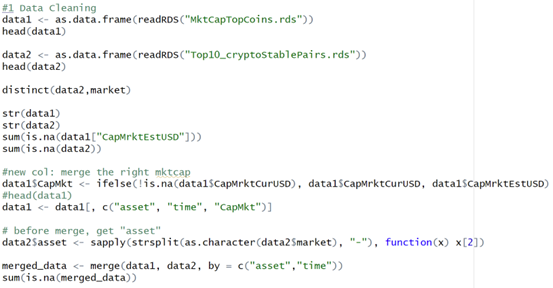
\includegraphics[width=0.7\textwidth]{2.png}
    \caption{Codes for Data Preparation - Cryptocurrencies Data} 
    \label{Codes for Data Preparation}
\end{figure}

To calculate the return of the value-weighted (market-capitalization-weighted) cryptocurrency index, daily log returns will be calculated as {\bf Equation 1} for each cryptocurrency based on its closing price and daily market-capitalization-weighted index return will be computed as {\bf Equation 2} as the weighted sum of the log daily returns for each cryptocurrency, weighted by shares of their market capitalizations on the date. {\bf Figure 3} shows the code in R for this procedure.

\[
\text{log\_daily\_return} = \log\left(\frac{\text{price\_close}}{\text{previous day price\_close}}\right) \tag{Equation 1}
\]

\begin{figure}[h]
    \centering
    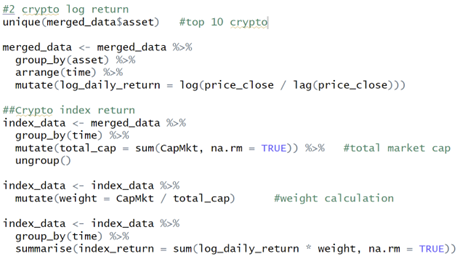
\includegraphics[width=0.7\textwidth]{3.png}
    \caption{Codes for Calculation of the Value-Weighted Cryptocurrency Index Return} 
    \label{Codes for Calculation of the Value-Weighted Cryptocurrency Index Return}
\end{figure}

\[
\text{index\_return} = \sum (\text{log\_daily\_return} \times \text{weight}) \tag{Equation 2}
\]
{\bf Figure \ref{Market-Capitalization-Weighted Index Return}} and {\bf Figure \ref{Market-Capitalization-Weighted Index Value}} shows the Market-Capitalization-Weighted Index Return and the Market-Capitalization-Weighted Index Value (with a base of 100 on 17th August 2017), respectively. These plots together provide insights into the daily fluctuations and longer-term trends in the top cryptocurrency market. The index return plot shows the day-to-day variability, while the index value plot demonstrates how the overall market capitalization changes cumulatively over time.

\begin{figure}[h]
    \centering
    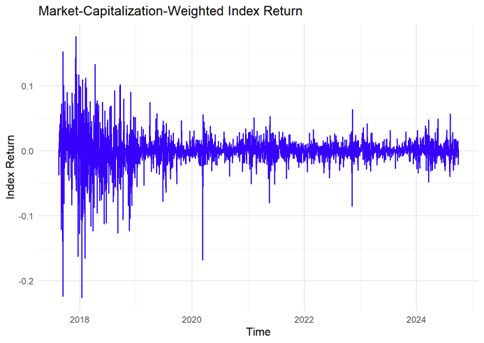
\includegraphics[width=0.7\textwidth]{4.png}
     \caption{Daily Returns of a Hypothetical Index based on the Market Capitalization}
    \label{Market-Capitalization-Weighted Index Return}
\end{figure}
\begin{figure}[h]
    \centering
    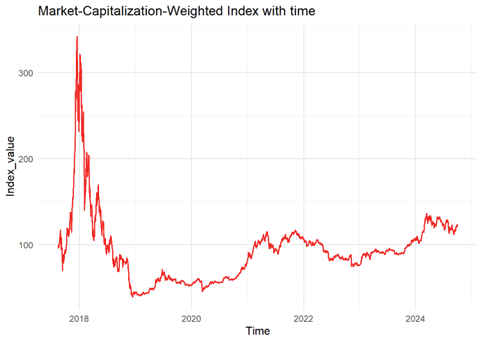
\includegraphics[width=0.7\textwidth]{5.png}
     \caption{The Index Value of the Market-Capitalization-Weighted Index}
    \label{Market-Capitalization-Weighted Index Value}
\end{figure}

\hypertarget{Set Benchmark: Risk-free and S\&P500}{%
\subsubsection{Benchmark: Risk-free and S\&P500}\label{Set Benchmark: Risk free and SP500}}
Han et al. (2021) used S\&P500, risk-free rates and value-weighted cryptocurrency index as benchmarks against cryptocurrency factor portfolios. Thus, this project combines the other two benchmarks' data with the value-weighted cryptocurrency index return constructed as {\bf Section 5.2.1} to compare the performance of cryptocurrencies with traditional financial benchmarks of risk-free rates and S\&P500. 

As shown in {\bf Figure 5}, the S\&P 500, the value-weighted cryptocurrency index and risk-free rates show no dominance over each other. Besides, the results by Han et al. (2021) indicated these three benchmarks yielded similar outcomes. To simplify the process, this project sets the S\&P 500 as the only benchmark against cryptocurrency factor portfolios, assuming that dominance over the S\&P 500 will indicate dominance over others.  


\begin{figure}[h]
    \centering
    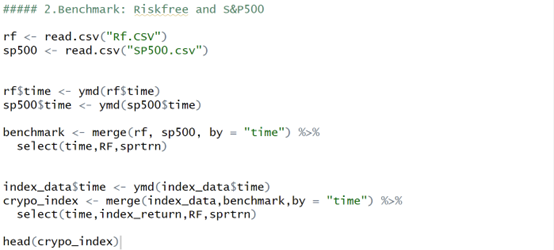
\includegraphics[width=0.7\textwidth]{6.png}
    \label{fig:example}
\end{figure}
\begin{figure}[h]
    \flushleft
    \hspace{2em}
    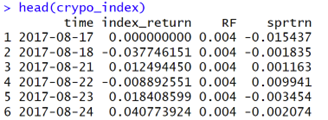
\includegraphics[width=0.5\textwidth]{7.png}
    \label{fig:example}
\end{figure}


\hypertarget{ECDFs Calculating}{%
\subsubsection{ECDFs Calculating}\label{ECDFs Calculating}}

To calculate the Empirical Cumulative Distribution Functions (ECDFs) for the S\&P 500 returns (sp\_cdf), risk-free rate (rf\_cdf), and the crypto index returns (crypto\_cdf), an ECDF function is applied to return the cumulative probability up to a given value in the input data. For example, for a value x, the ECDF function returns the proportion of data points that are less than or equal to x. The plot compares the distributions of returns for the crypto index, S\&P 500, and the risk-free rate. By observing the shape of the CDFs, we can identify which asset is riskier (steeper increases indicate more concentrated values), which has more variability, and how they perform relative to each other.

\begin{figure}[H]
    \centering
    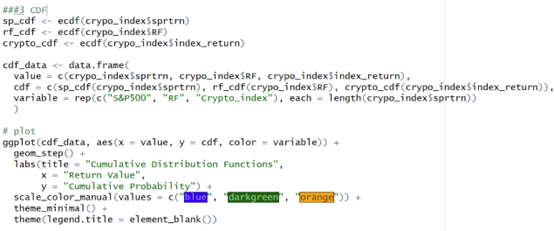
\includegraphics[width=0.8\textwidth]{8.png}
    \label{fig:example}
\end{figure}
\begin{figure}[H]
    \centering
    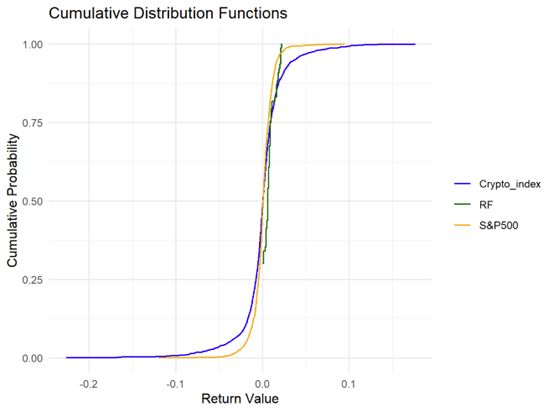
\includegraphics[width=0.7\textwidth]{9.png}
    \caption{Cumulative Distribution Function for Risk free, SP500 and crypto index}
    \label{fig:example}
\end{figure}
\begin{figure}[H]
    \centering
    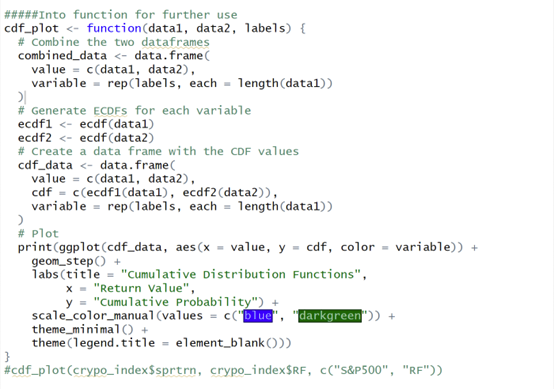
\includegraphics[width=0.7\textwidth]{10.png}
    \label{fig:example}
\end{figure}

Then the cdf\_plot function is introduced as a reusable tool for comparing the distribution of two different sets of data. This helps the later modeling of AFSD and ASSD. 

\hypertarget{AFSD \& ASSD}{%
\subsubsection{AFSD \& ASSD}\label{AFSD ASSD}}
Almost Stochastic Dominance is a concept used in decision theory and finance to compare distributions of returns or outcomes, allowing for some tolerance of violations in the preference ordering. To test whether AFSD and ASSD exist, we calculate the ratio of violation area over the total enclosed area for each portfolio and compare these ratios ($\epsilon_1$ for AFSD and $\epsilon_2$ for ASSD) to determine if they are lower than AFSD (5.9%) and ASSD (3.2%), showing that they meet the requirement. 

For AFSD, the FSD violation range is given by:
\[
R_1(F_H, F_L) = \{s \in (r_1, r_2): F_L(s) < F_H(s)\}
\]

The empirical violation area is defined as:
\[
\epsilon_1 = \frac{\int_{R_1} \left[F_H(s) - F_L(s)\right] ds}{\int_{\text{min}}^{\text{max}} \left[F_H(s) - F_L(s)\right] ds}
\]

If $\epsilon_1 < 5.9\%$, AFSD exists.
\begin{figure}[H]
    \centering
    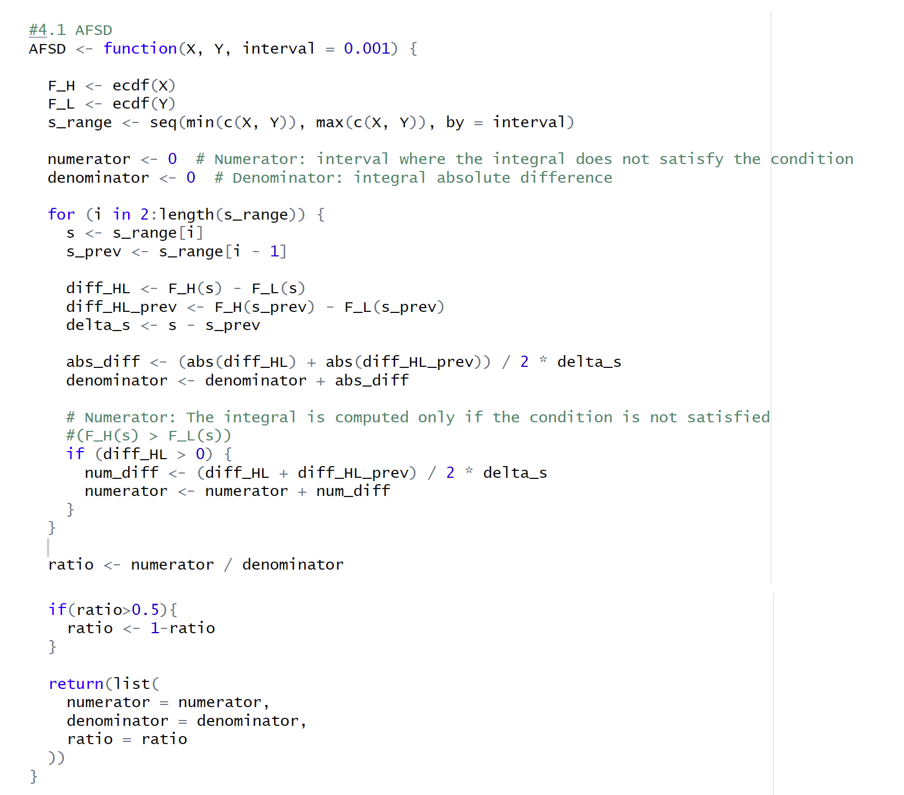
\includegraphics[width=0.7\textwidth]{11.png}
    \label{fig:example}
\end{figure}
For ASSD, the SSD violation range is given by:
\[
R_2(F_H, F_L) = \left\{ s \in (F_H, F_L) : \int_0^r \left[ F_L(s) - F_H(s) \right] ds < 0 \right\}
\]

The empirical violation area is defined as:
\[
\epsilon_2 = \frac{\int_{R_2} \left[ F_H(s) - F_L(s) \right] ds}{\int_{\text{min}}^{\text{max}} \left[ F_H(s) - F_L(s) \right] ds}
\]

If $\epsilon_2 < 3.2\%$, ASSD exists.
\begin{figure}[H]
    \centering
    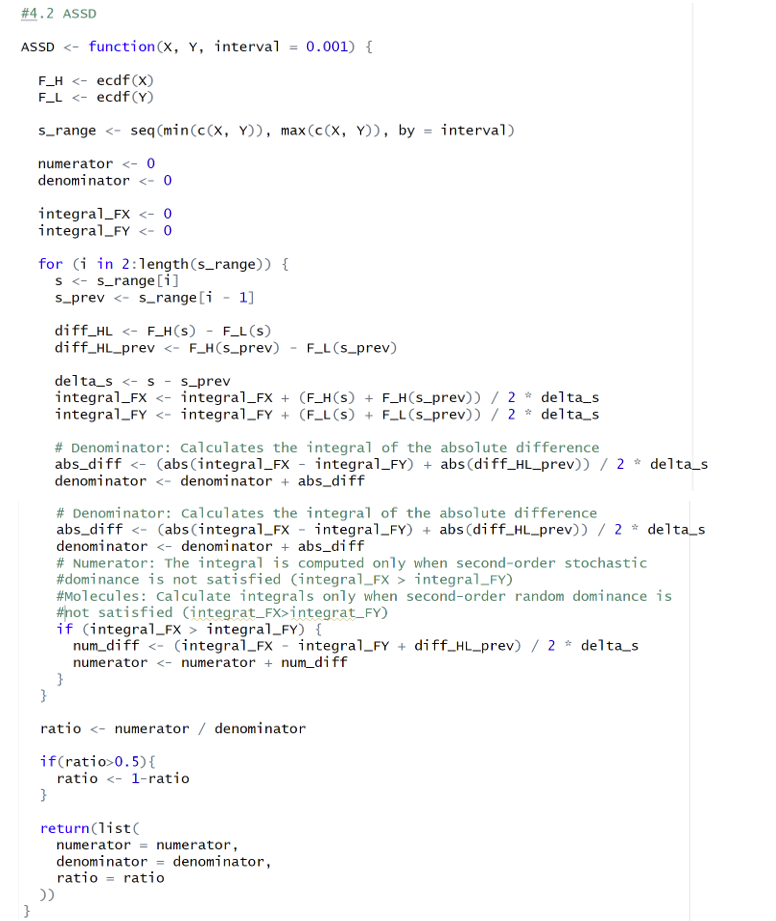
\includegraphics[width=0.7\textwidth]{12.png}
    \label{fig:example}
\end{figure}
\hypertarget{Factor Calculation}{%
\subsubsection{Factor Calculation}\label{Factor Calculation}}


Asset characteristics are calculated based on 22 factors related to key aspects of size, momentum, volume, and volatility.

\paragraph{Momentum Factors:}
Momentum measures the rate of price change over time and is calculated using lagged values of the asset prices. 
\begin{itemize}
    \item \textbf{Lagged Values}: Lag1, Lag2, Lag3, Lag4, Lag8 represent the asset’s lagged prices over different time periods (7, 14, 21, 28, and 56 days). 
    \item \textbf{Momentum (mom)}: These factors are calculated as the difference between the current price and the lagged prices over different time horizons (mom1, mom2, mom3, mom4, mom8). This shows how much the asset’s price has changed over those time intervals. 
\end{itemize}

\paragraph{Volatility Factors:}
Volatility factors measure the risk and dispersion of returns over various time periods. 
\begin{itemize}
    \item \textbf{Standard Deviation (std)}: Standard Deviation are calculated over rolling windows of 7, 14, 21, 28, and 56 days (std1, std2, std3, std4, std8). This provides an estimate of how much the price fluctuates within the specified period. 
    \item \textbf{Risk-Adjusted Momentum (rmom)}: Momentum is adjusted by dividing by the corresponding standard deviation to account for risk. These are also calculated over different time windows (rmom1, rmom2, rmom3, rmom4, rmom8)
\end{itemize}

\paragraph{Size Factors:}
The size of an asset is generally measured by its market capitalization (\textit{CapMkt}), which is the product of price and the number of shares outstanding. 
\begin{itemize}
    \item \textbf{Log-Price (lprc)}: The natural logarithm of the price to stabilize the variance. 
    \item \textbf{Max Price (maxprc)}: The maximum price observed over a rolling 7-day window. 
\end{itemize}

\paragraph{Volume Factors:}
Volume factors reflect the trading activity and liquidity of the asset. 
\begin{itemize}
    \item \textbf{Log-Volume (vol)}: The natural logarithm of the average volume over a rolling 7-day window. 
    \item \textbf{Volume-Price Product (volprc)}: The product of volume and price, representing the total traded value. 
    \item \textbf{Volume-Scaled Price (volscale)}: Volume-price product divided by market capitalization to assess the liquidity relative to the asset size. 
\end{itemize}

The process will build portfolios described in {\bf Setion 5.2.6} and compare the portfolios based on weekly return calculations to evaluate if one strategy or factor dominates another. 

\paragraph{Quantile:}
Quantile formation involves sorting assets based on factor values and dividing them into equalsized groups. This method is used to classify assets according to their factor characteristics. For each factor, the assets are divided into five quantiles, and this categorization helps analyze the performances of portfolios 
constructed from each quantile. 

By categorizing the assets into quantiles for each of these factors, the code enables analysis of portfolio returns, risks, and other metrics. Quantile-based sorting allows for examining if certain factor characteristics (e.g., high momentum or low volatility) result in superior performance.



\hypertarget{Portfolio Building}{%
\subsubsection{Portfolio Building}\label{Portfolio Building}}
This project then analyzes financial portfolios, focusing on constructing portfolios based on different factors such as size, momentum, volatility, and volume. Portfolio returns are calculated using the value-weighted methods as Han et al. (2021), with the ultimate goal of assessing the performance of different quantile-based portfolios.

\textbf{Step 1: Portfolio Building}\\
Portfolios are built based on different factors, such as size, momentum, volatility, and volume, combined with returns of the following week.

\textbf{Step 2: Value-Weighted Portfolio Calculation}\\
This project calculates returns for a value-weighted portfolio as the replicated paper did. The weights of each asset (weights\_port) are calculated by dividing the market value of each asset by the total market value for the period. This normalization ensures that the sum of the weights equals 1. If holding\_period is 1, it uses the default returns (e.g., 1-week weekly returns). For longer holding periods, it uses cumulative returns over that period.
This approach ensures that larger assets (by market value) have a more significant impact on the portfolio's returns, following a value-weighted methodology. 

\textbf{Step 3: Summary Calculations for Different Factors}\\
The average returns are calculated for different quantiles (1 to 5) across various factors.

\textbf{The Quantile-Based Long/Short Strategy:}
\begin{itemize}
    \item The project divides each factos into five quantiles and the {\bf Table 2} shows the returns for each quantile from 1 to 5.
    \item \textbf{Long Positions}: Assets in the top quantile (5).
    \item \textbf{Short Positions}: Assets in the bottom quantile (1).
    \item The column (5-1) computes portfolio returns as the difference between the returns from long and short positions.
\end{itemize}

\begin{table}[H]
    \centering
    \caption{Quantiles for the factors}
    \begin{tabular}{c}
        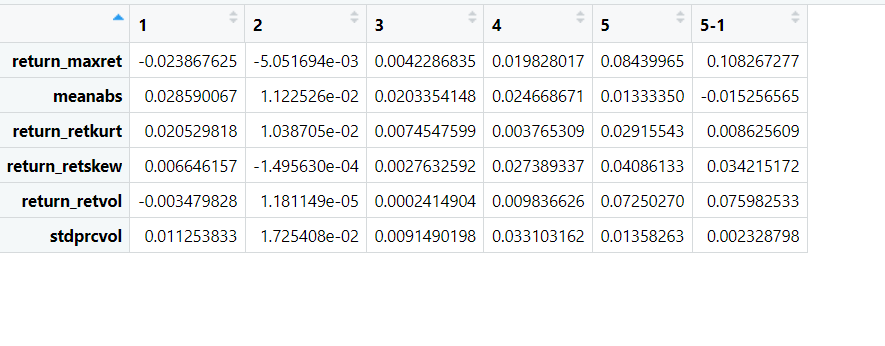
\includegraphics[width=0.7\textwidth]{21.png} \\
        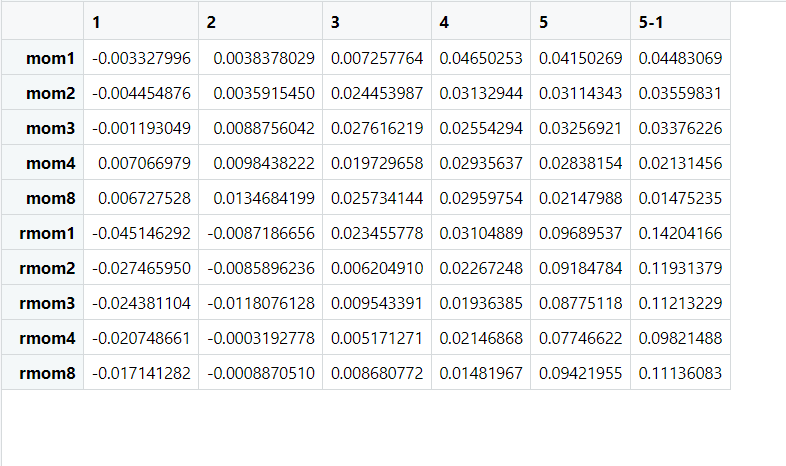
\includegraphics[width=0.7\textwidth]{22.png} \\
        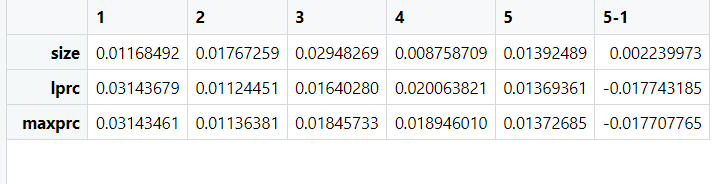
\includegraphics[width=0.7\textwidth]{23.png} \\
        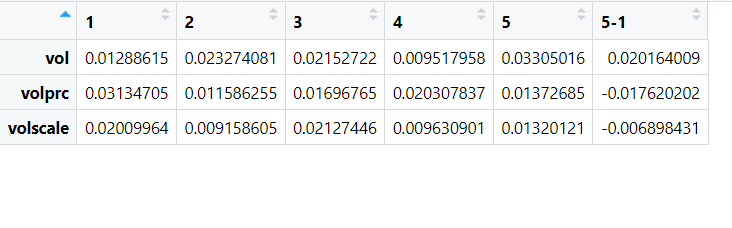
\includegraphics[width=0.7\textwidth]{24.png} \\
    \end{tabular}
    \label{fig:example}
\end{table}

\hypertarget{AFSD and ASSD testing and plotting}{%
\subsubsection{AFSD and ASSD testing and plotting}\label{AFSD and ASSD testing and plotting}}

This analysis involves testing AFSD and ASSD across different factors and holding periods, using log returns for the S\&P 500 index as a benchmark.

\textbf{Step 1: Set the Benchmarks of Risk-Free and S\&P 500}\\
Firstly, the following code shows ways to read and prepare weekly log return data for the S\&P 500. This step converts the Date column to a Date format, computes the weekly log returns, and adjusts the dates.
\begin{figure}[H]
    \centering
    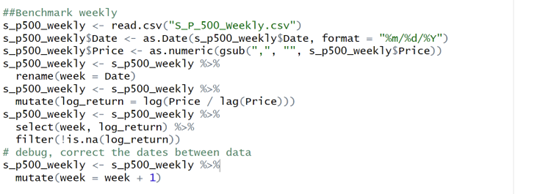
\includegraphics[width=0.6\textwidth]{15.png}
    \label{fig:example}
\end{figure}
\textbf{Step 2: AFSD and ASSD Testing}\\
Different factor-based long-short portfolio returns will be compared with the S\&P 500 returns. AFSD and ASSD are used to measure the dominance relationships between the long-short portfolio performance and the benchmark.\\
The following codes take the size based portfolios as an example to calculate the AFSD and ASSD. Same techniques and methodologies will be applied to momentum, volatility and volume based portfolios.



\begin{figure}[H]
    \centering
    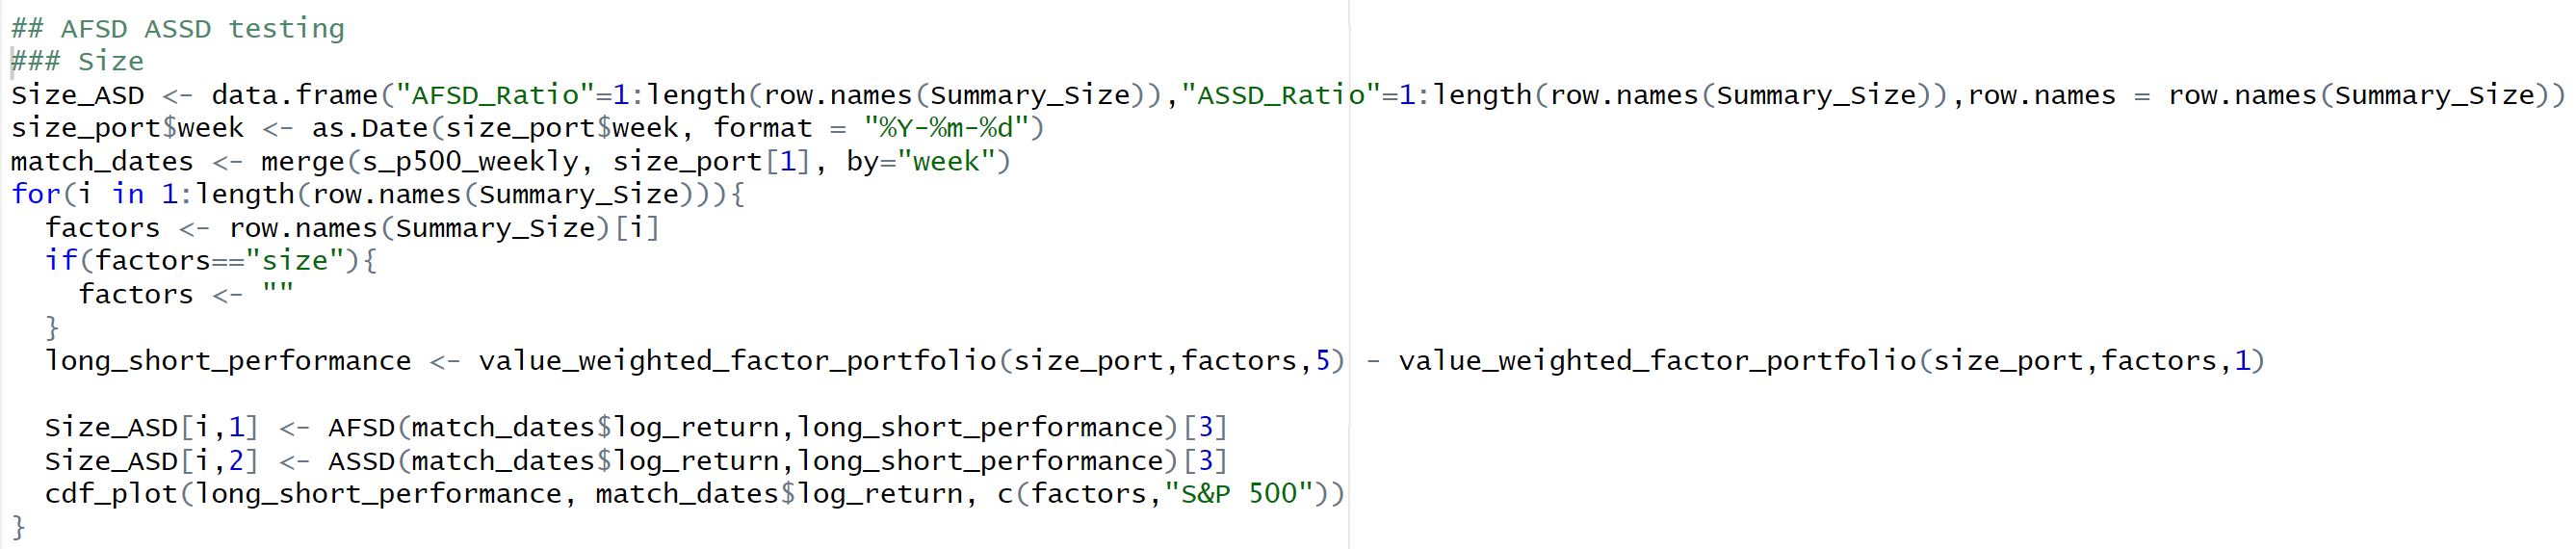
\includegraphics[width=0.9\textwidth]{19.png}
    \label{fig:example}
\end{figure}

\textbf{Step 3: Factor Analysis by Holding Periods}\\
After constructing and analysing portfolios with a holding period of 1 week, this project extends the holding period similar to Han et al. (2021) and analyzes portfolios' performances over these holding periods (4 weeks, 13 weeks, 26 weeks, 52 weeks, and 78 weeks).
The following codes take the size based portfolios as an example to calculate the portfolios performances for holding periods longer than one week. Same techniques and methodologies will be applied to momentum, volatility and volume based portfolios.
\begin{figure}[H]
    \centering
    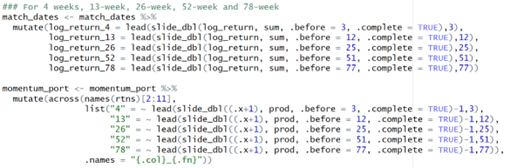
\includegraphics[width=0.6\linewidth]{20.png}
    \label{fig:enter-label}
\end{figure}



\begin{figure}[H]
    \centering
    \begin{subfigure}{0.45\textwidth}
        \centering
        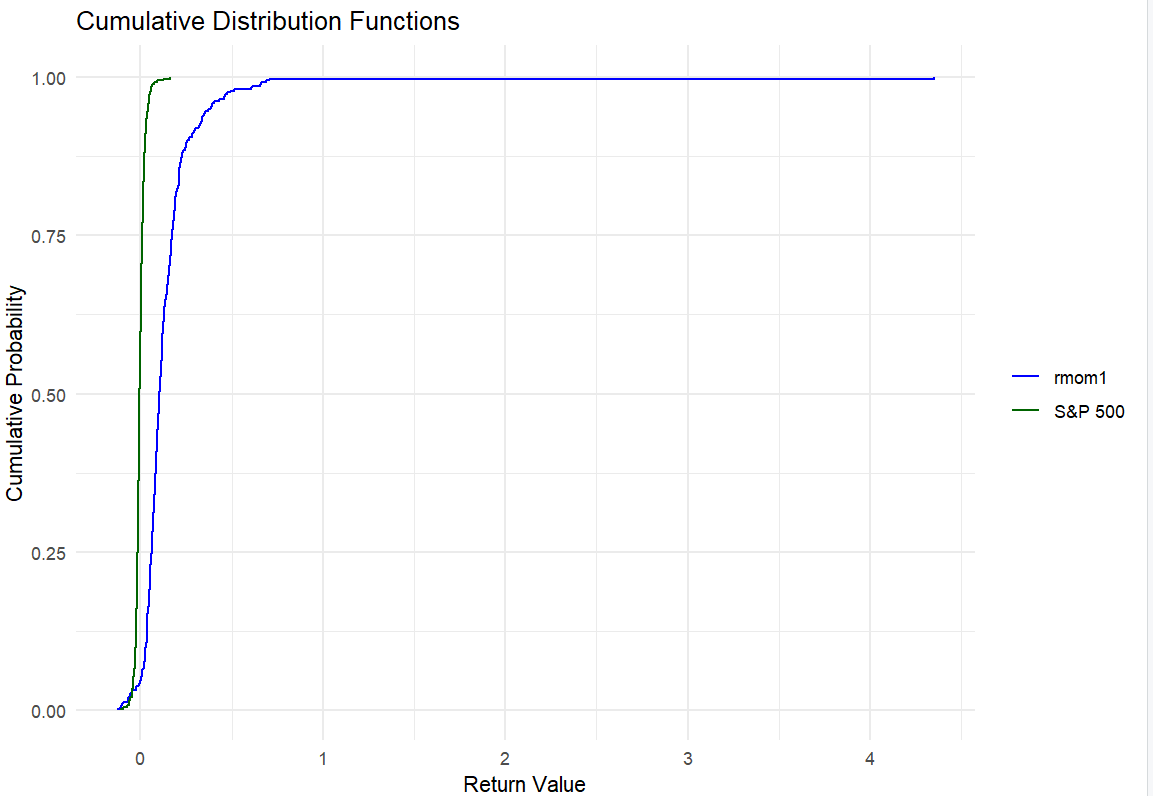
\includegraphics[width=\textwidth]{25.png}
        \caption{mom1}
        \label{fig:image25}
    \end{subfigure}
    \hspace{0.05\textwidth}
    \begin{subfigure}{0.45\textwidth}
        \centering
        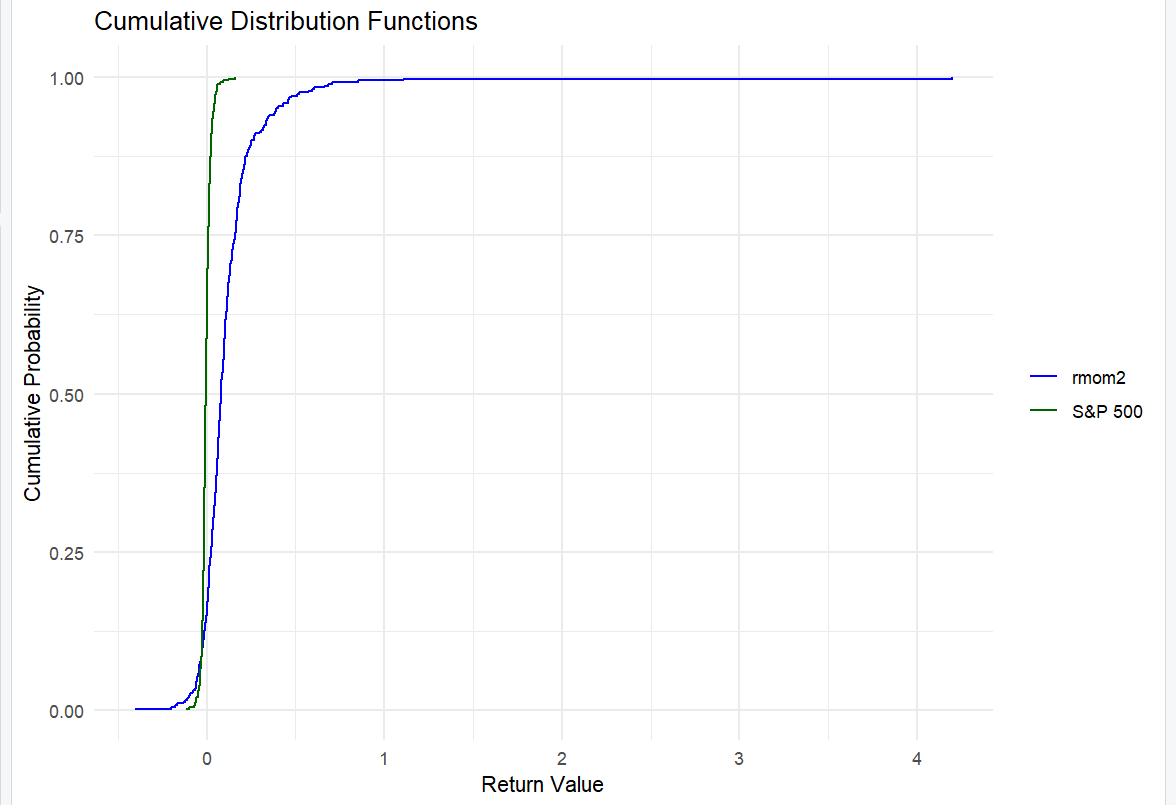
\includegraphics[width=\textwidth]{26.png}
        \caption{mom2}
        \label{fig:image26}
    \end{subfigure}

    \begin{subfigure}{0.45\textwidth}
        \centering
        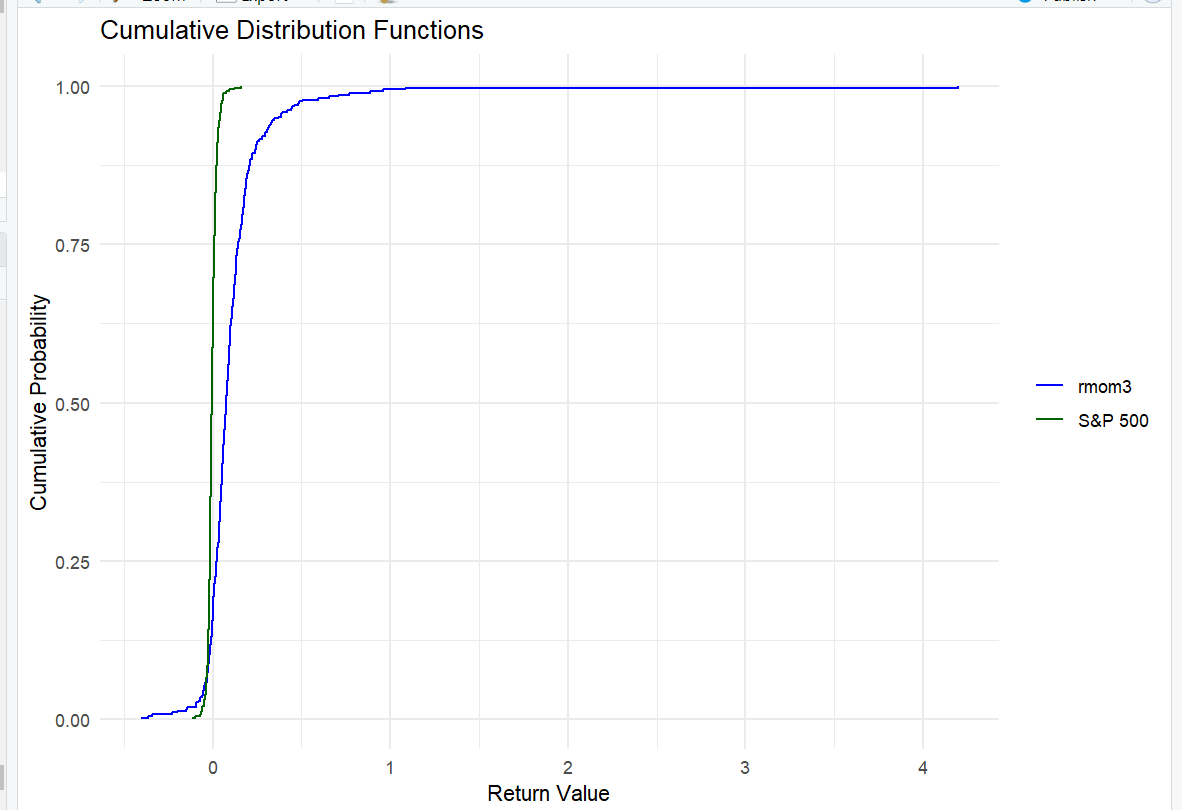
\includegraphics[width=\textwidth]{27.png}
        \caption{mom3}
        \label{fig:image27}
    \end{subfigure}
    \hspace{0.05\textwidth}
    \begin{subfigure}{0.45\textwidth}
        \centering
        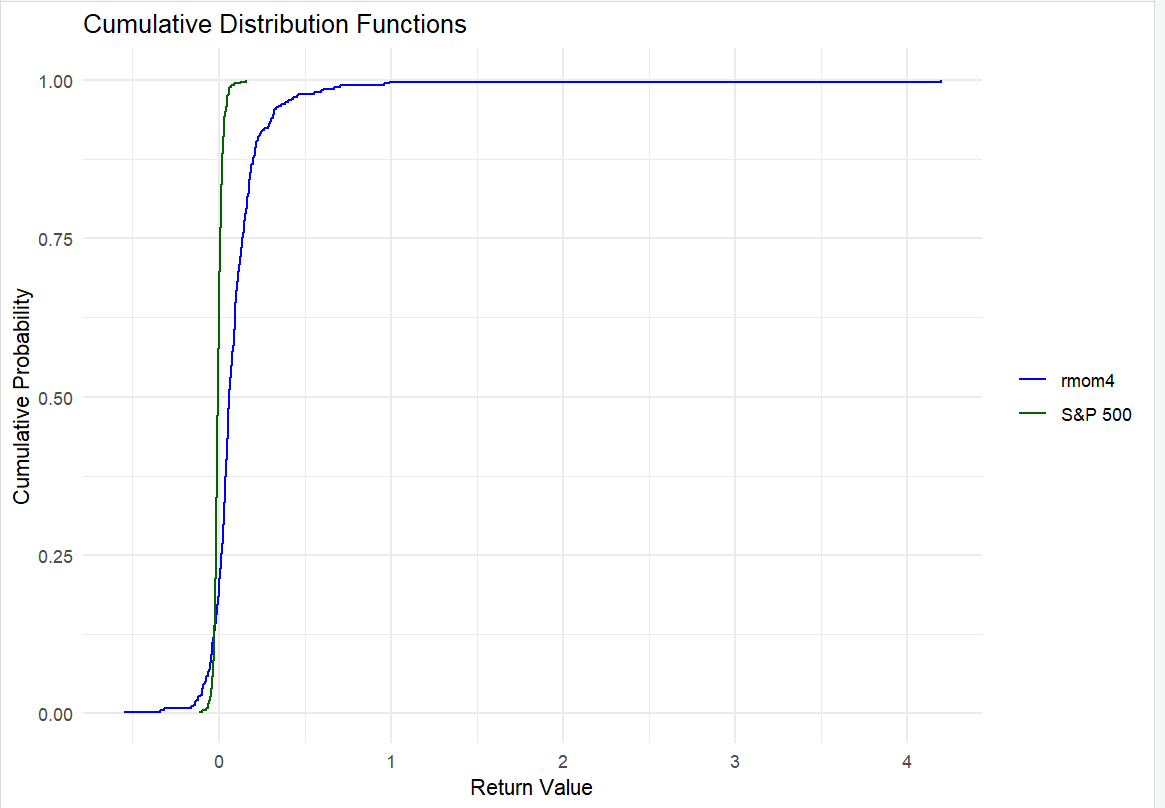
\includegraphics[width=\textwidth]{28.png}
        \caption{mom4}
        \label{fig:image28}
    \end{subfigure}

    \begin{subfigure}{0.45\textwidth}
        \centering
        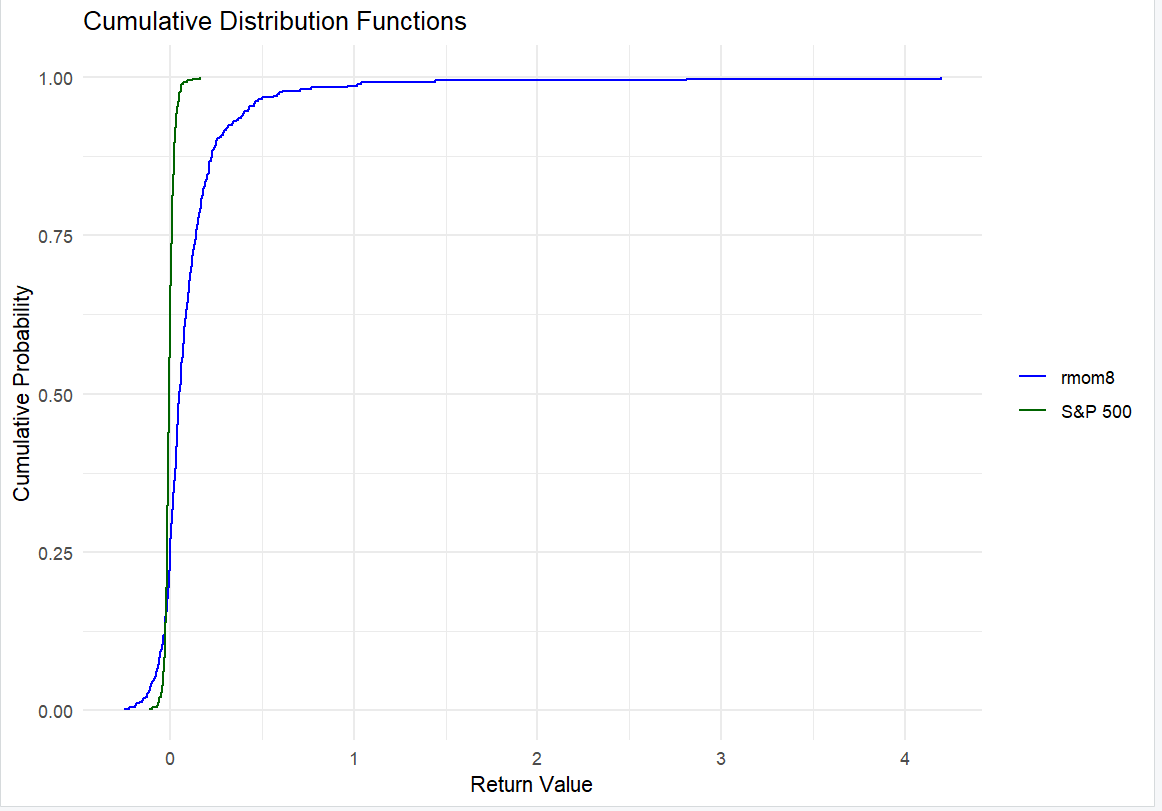
\includegraphics[width=\textwidth]{29.png}
        \caption{mom8}
        \label{fig:image29}
    \end{subfigure}
    \hspace{0.05\textwidth}
    \begin{subfigure}{0.45\textwidth}
        \centering
        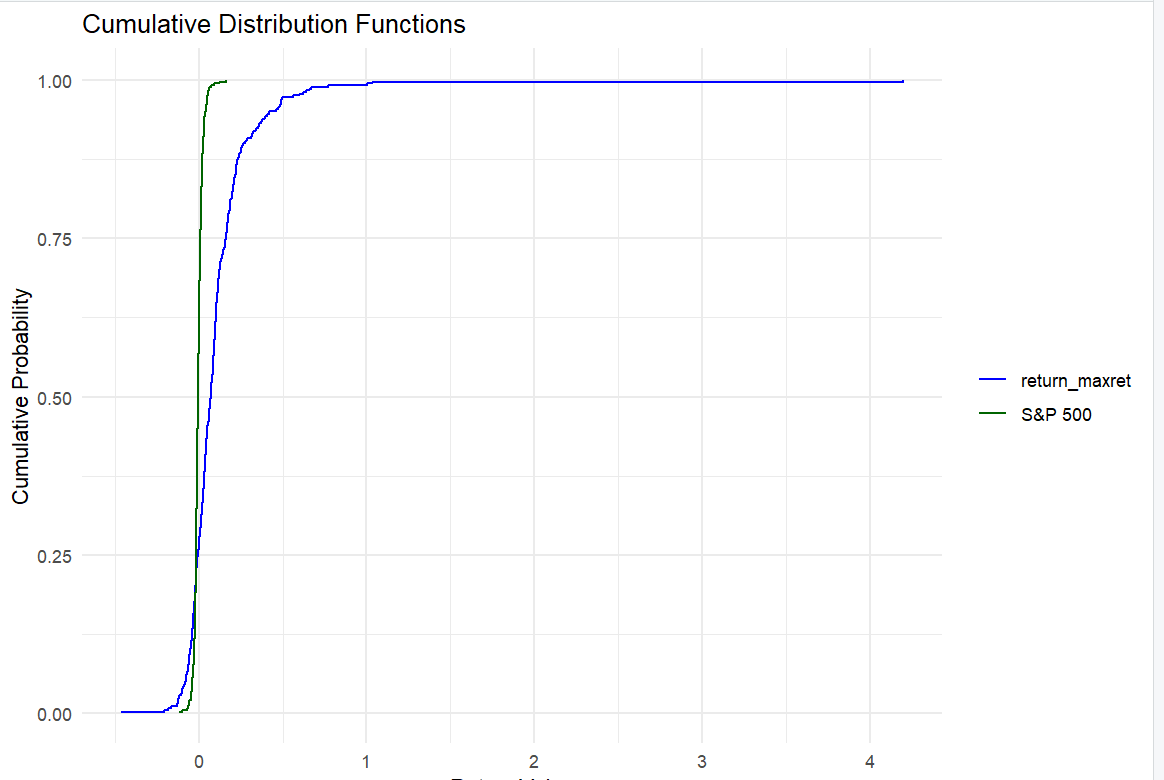
\includegraphics[width=\textwidth]{30.png}
        \caption{maxret}
        \label{fig:image30}
    \end{subfigure}

    \begin{subfigure}{0.45\textwidth}
        \centering
        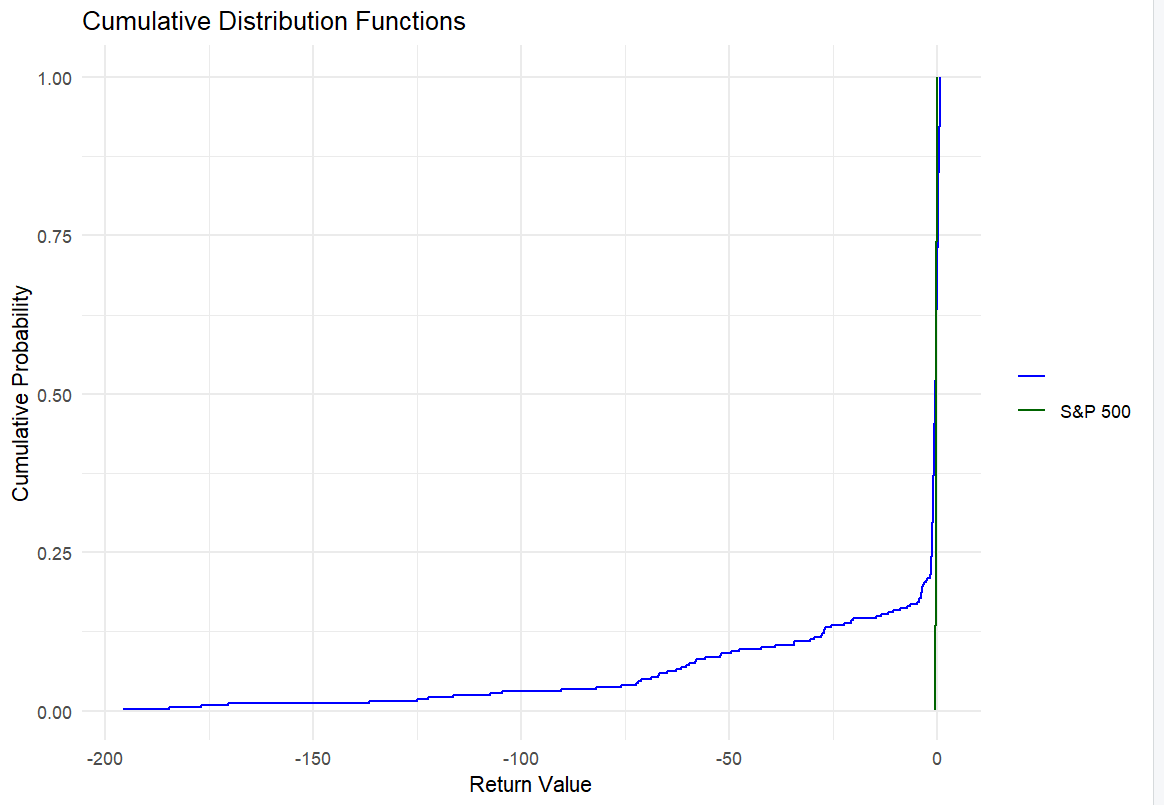
\includegraphics[width=\textwidth]{31.png}
        \caption{marketcap-52weeks}
        \label{fig:image31}
    \end{subfigure}
    \hspace{0.05\textwidth}
    \begin{subfigure}{0.45\textwidth}
        \centering
        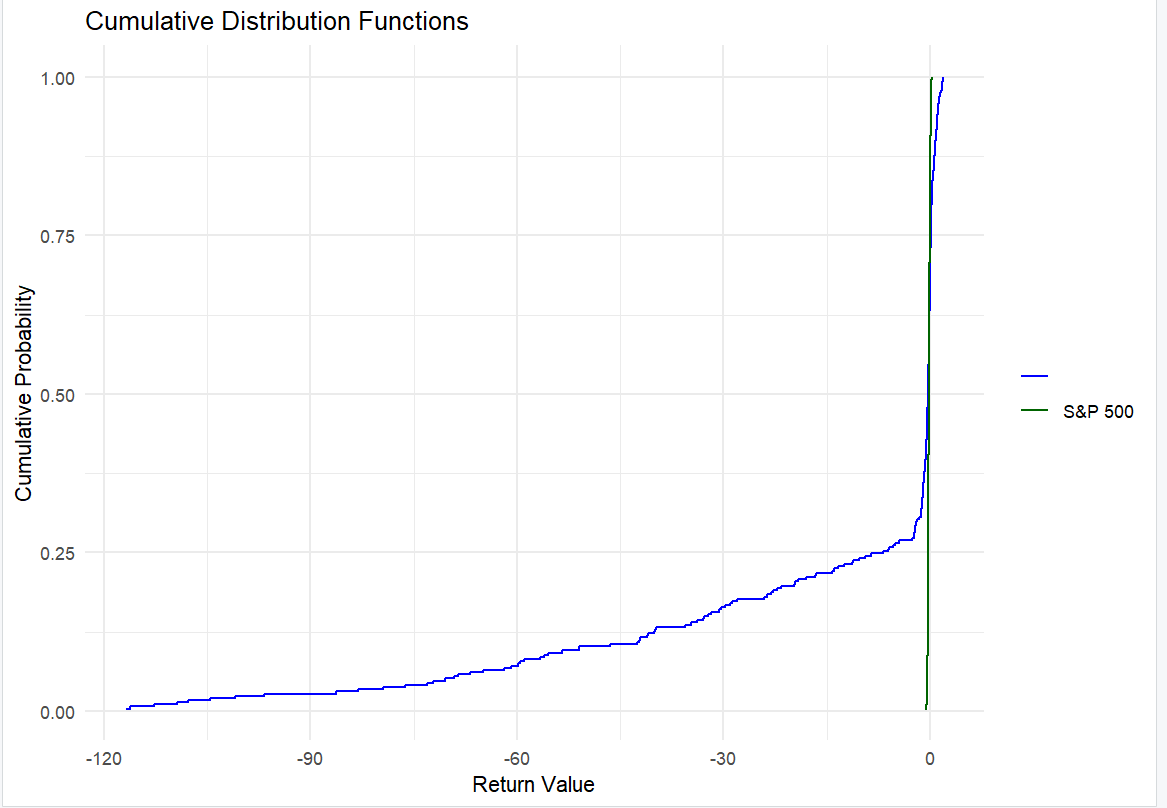
\includegraphics[width=\textwidth]{32.png}
        \caption{marketcap-78weeks}
        \label{fig:image32}
    \end{subfigure}

    \caption{CDF of factor portfolios against benchmark}
    \label{fig:multiimages}
\end{figure}

\textbf{Step 4: Identifying Dominant Factors}\\
After calculations of $\epsilon_1$ for AFSD and $\epsilon_2$ for ASSD mentioned in {\bf Section 5.2.4} for each long-short portfolio for each factor, the following codes test whether factors exhibit dominance according to AFSD and ASSD criteria for a specified holding period. This project uses similar thresholds (5.9\% for AFSD and 3.2\% for ASSD) to Han et al. (2021) as mentioned before in {\bf Section 2} to determine dominance. The {\bf Figure 6} shows AFSD graphs for the dominant factors with corresponding dominant holding periods. Suggested by Han et al. (2021), the direction of dominance of long-short portfolios will not be a matter, because switching the long-short quantiles will solve this issue. Based on the data used by this project, rmom1 - rmom8 and maxret shows dominance against S\&P 500 for the holding period of one week, and marketcap shows dominance the holding periods of 52 weeks and 78 weeks.
\begin{figure}[H]
    \centering
    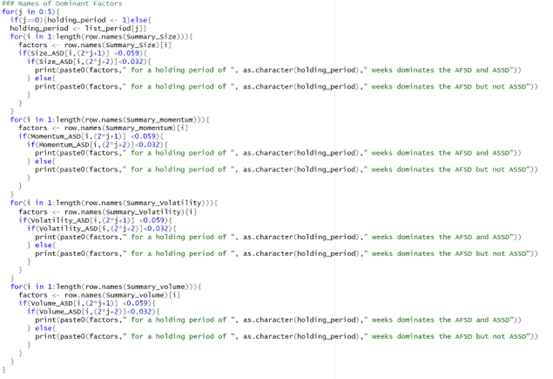
\includegraphics[width=0.8\textwidth]{16.png}
    \label{fig:example}
\end{figure}

\hypertarget{Contributions of Dominances}{%
\subsection{Contributions of Dominances}\label{Contributions of Dominances}}

After identifying the dominant factors, this project tries to figure out whether long-legs, short-legs or both contribute to the dominance of these dominant factors.

The following codes take rmom1 as an example, creating factor-based long-only, short-only and long-short portfolios. The codes are used to create a long-only portfolio by investing in assets in the top quantile (5), a short-only portfolio by shorting assets in the bottom quantile (1) and a long-short portfolio by combining two portfolios. Same techniques will be applied to rmom2 - rmom8 for one week investment horizon and CapMkt for 52-week and78-week investment horizons. Then, the AFSD and ASSD are utilized to calculate the Almost Stochastic Dominance statistics to test whether:
\begin{itemize}
    \item The long-only portfolio dominates the benchmark.
    \item The short-only portfolio dominates the benchmark.
    \item The short-only portfolio dominates the long-only portfolio.
    \item The short-only portfolio dominates the long-short portfolio.
    \item The long-only portfolio dominates the long-short portfolio.
\end{itemize}
\begin{figure}[H]
    \centering
    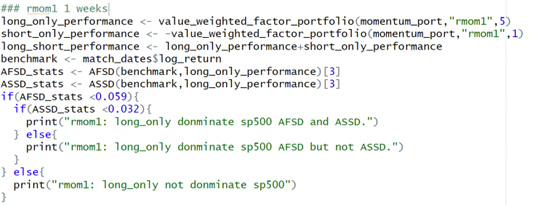
\includegraphics[width=0.7\textwidth]{17.png}
    \label{fig:example}
\end{figure}


\subsubsection{Results}
\begin{itemize}
    \item \textbf{Momentum Factors (rmom1, rmom3, rmom4, rmom8):}
    \begin{itemize}
        \item \textbf{Long-Only vs. S\&P 500}: For all momentum factors tested, the long-only strategy does not dominate the S\&P 500 for both AFSD and ASSD, indicating that a long-only approach may not outperform the benchmark.
        \item \textbf{Short-Only vs. S\&P 500}: Similarly, the short-only strategy fails to dominate the S\&P 500, suggesting it does not provide better returns than the benchmark.
        \item \textbf{Short-Only vs. Long-Only}: In each case, the short-only strategy shows a significant dominant relationship with the long-only strategy for both AFSD and ASSD criteria. After checking the patterns of each portfolio, this project suggests that shorting low-ranked assets yields inferior performance than buying high-ranked assets in the momentum context.
        \item \textbf{Short-Only vs. Long-Short}: The short-only strategy also shows a significant dominant relationship with the long-short strategy across all momentum factors, indicating that pure shorting is significantly less effective than combining long and short positions.
        \item \textbf{Long-Short vs. Long-Only}: In some cases (like rmom1), the long-short strategy shows a significant dominant relationship with the long-only strategy, suggesting that including short positions worsens performance over a pure long strategy.
    \end{itemize}
     Generally speaking, the insignificant dominant relationships for long-leg and short-leg with the benchmark, S\&P 500, are a result of huge left-tail losses. However, this effect will be mitigated when combining two legs, of which a negative correlation between two legs may be a cause. Besides, long-leg consistently yields better performances, potentially indicating that long-leg contributes more to the long-short strategies.
    \item \textbf{Size Factor for Longer Holding Periods:}
    \begin{itemize}
        \item As suggested by the patterns of AFSD between CapMkt and the benchmark, shorting the large-size cryptocurrencies (quantile 1) and longing the small-size cryptocurrencies (quantile 5) will yield superior returns than S\&P 500. Thus, the long-only strategy here will refer to longing the small-size cryptocurrencies and the short-only strategy will refer to shorting the large-size cryptocurrencies (quantile 1).
        \item For both 52-week and 78-week investment horizons, the long-only strategy dominates the S\&P 500 in both AFSD and ASSD for a 52-week holding period, while the short-only strategy does not dominate the S\&P, indicating that the long-leg contributes more than the short-leg due to huge right-tail positive returns, even though the short leg will further improve the right-tail positive returns by a small extent.
    \end{itemize}
\end{itemize}

These results highlight the importance of the contributions of the long legs, even though the short legs will improve the performances by either mitigating huge left-tail losses or improving the huge right-tail returns.

\hypertarget{future-work}{%
\section{Future Work}\label{future-work}}



The original paper is vulnerable to overfitting issues. Firstly, because a large number of factors and several investment horizons were adopted, the dominance factors may be detected by chance. This issue was mitigated by adopting a six-year panel data with 400 cryptocurrencies. However, this project replicates those factors and methodologies with a significantly small dataset, which will be much more vulnerable to overfitting. Secondly, a six-year observation may not be enough to witness a full picture of the market cycle. The resulting dominance of the original paper may be a result of weak stock market conditions, such as that in 2018, or a strong cryptocurrency market. Given the high volatility of cryptocurrency assets, it is unclear whether a portfolio constructed from historical data will continue to perform well under new future conditions. Furthermore, the original paper constructed portfolios by allowing both buying and short-selling without costs, but it disregards real-world transaction costs and short-selling constraints, which could also impact the portfolio's performance.

Future research could extend the analysis by examining longer observation horizons to include a full market cycle, employing more cryptocurrencies and incorporating different asset benchmarks, such as commodities or real estate, to better understand the performance of cryptocurrency factors over time and across a broader investment landscape. Up-to-date data and a larger number of cryptocurrencies will reduce the possibility of overfitting and provide more reliable information about the current market. Additionally, investigating the impact of various market conditions (e.g., bull vs. bear markets) on factor dominance could provide insights into the conditional performance of cryptocurrency investments. Besides, setting constrains, such as  transaction costs and short-selling limitations, will gain more reliable results for real-world strategies.



\hypertarget{conclusions}{%
\section{Conclusions}\label{conclusions}}

This analysis employs non-parametric almost stochastic dominance (AFSD and ASSD) to assess the performance of various portfolio strategies based on different factors, including momentum, size, volume and volatility. It aims to determine if these strategies can outperform the S\&P 500 benchmark over different time horizons, ranging from 1 to 78 weeks. 

Our findings indicate that risk-adjusted momentum-based strategies (rmom1, rmom3, rmom4, and rmom8) exhibit dominant factors in the short term (1 week). Furthermore, long-short strategies generally perform better than long-only strategies, particularly for short-term momentum factors. In the longer term (52 and 78 weeks), the size factor (CapMkt) shows significant dominance over the benchmark. Although a few dominant factors were found,  the number was significantly less than that found by the original paper, which found nine dominant factors across 26-week to 78-week holding horizons. This may indicate a changing market environment, an overfitting issue of the original paper, or a small dataset of this project.

After obtaining the dominant factors with corresponding dominant investment horizons, this project evaluates the relative contributions of long legs and short legs to long-short portfolios constructed by these dominant factors. This project gains similar results as the original paper, suggesting the long legs contribute more than the short legs. This result does not undervalue the importance of short legs, which improve the performances of long legs by either mitigating huge left-tail losses or improving the huge right-tail returns.  Especially, for short-term momentum strategies, long-only approaches do not dominate the benchmark, highlighting the importance of short legs in mitigating huge losses and the limitations of long-only strategy.

Further research should explore a large dataset with longer up-to-date observation horizons and more cryptocurrencies to mitigate overfiting and obtain more instructive information. Moreover, different benchmarks should be examinated to check the dominances cryptocurrency factor strategies across larger investment landscape. Thirdly, incorporating some real-world constraints into the investigation will be helpful to gain more practical guidances. 


\newpage

\begin{figure}
\centering

\includegraphics{cc_by_88x31.png}
\caption{CC-BY}
\end{figure}

\nocite{*}
\printbibliography[notkeyword=ignore]

\end{document}
